
\chapter{Preliminary Studies}
\label{Preliminary Studies}
\lhead{Chapter 3. \emph{Preliminary Studies}}

This chapter describes the studies made on relevant technologies and similar solutions and how they affected our design choices. 
Additionally, we examine two common development models and explain our reasons behind the choice of one instead of the other.

%-----------
% SECTION 1
%-----------

\section{Development Methodology}
\label{section:development-methodology}

Choosing an appropriate development process is vital to any software project.
It is a choice that has to be made early on because it will influence planning as well as many other activities. 
In this section we give a brief description of two common development methodologies we took into consideration
for our project and outline the factors that led to chose one instead of the other.

%-----------------------------------
%	SUBSECTION 1
%-----------------------------------
\subsection{Waterfall}
%of Waterfall is its requires tasks to be performed in a sequential order.

The Waterfall\cite{WaterfallModel} development process is a model proposed in the early 70's.
It divides the development cycle in seven distinct phases (see figure \ref{figure:waterfall-model}),
each one expected to produce extensive documentation.
It follows a strict, rigorous top-down approach where all phases of the process are carried out sequentially:
before moving to the next phase the preceding ones need to be entirely completed. The progress of the project
is seen as if 'flowing downwards' through the different phases, hence the name \textit{Waterfall}.
%The development cycle consists of seven 

\begin{figure}[h]
\begin{center}
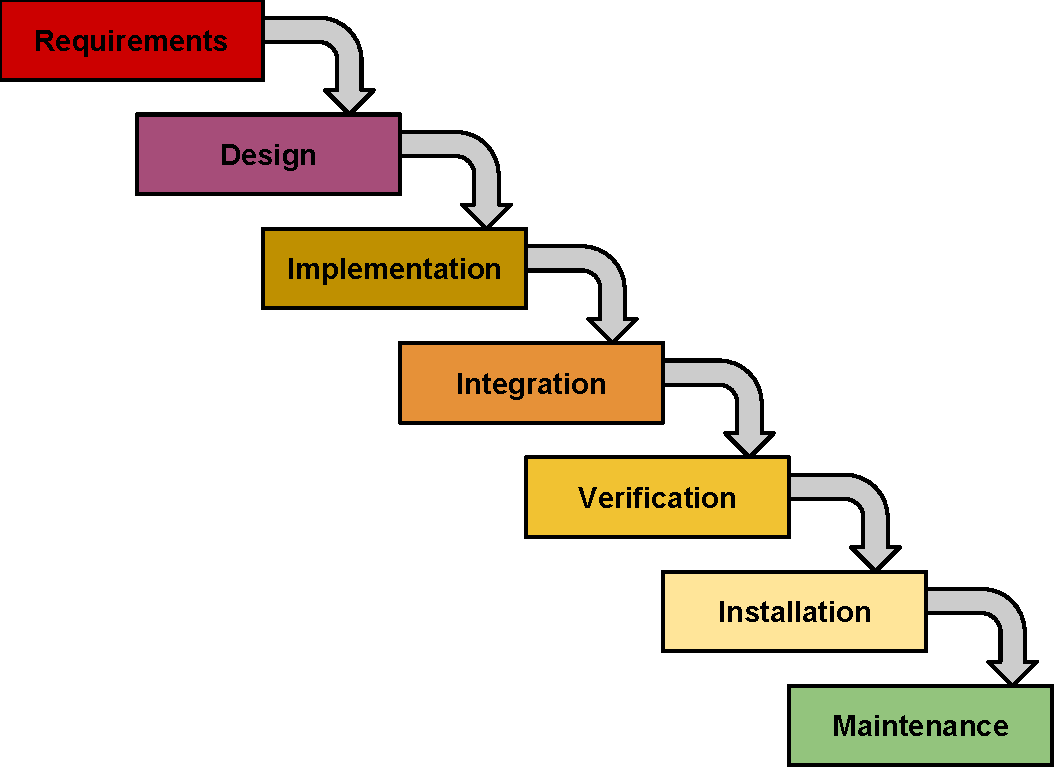
\includegraphics[scale=0.6]{../Figures/Waterfall-model.pdf}
\end{center}
\caption{Development cycle in Waterfall}
\label{figure:waterfall-model}
\end{figure}

The model is easily understandable, structured and disciplined.
The clear distinction between project phases make it easier to monitor the progress of the project.
However, adopting Waterfall in real software projects can be challenging because it requires to be able to
foresee, in the early stages of the project, any problem that could arise later on and plan accordingly.
This is often a very hard task which requires great insight and expertise.

Waterfall may be suited to large-scale, expensive projects where 'going back' on design choices is not an
option and requirements are clearly established early on and then 'set in stone'.
However, many software projects nowadays fail to meet these conditions.

%-----------------------------------
%	SUBSECTION 2
%-----------------------------------
\subsection{Scrum Model}
%cite http://www.mountaingoatsoftware.com/agile/scrum

Scrum is an emerging agile development process which is mostly used in software development.
The Scrum approach, which could be described as both iterative and incremental, consists of multiple
sprints which last from two to four weeks. Sprints begin with a planning meeting and conclude with a review meeting.

During the sprint planning meeting team members produce a \emph{sprint backlog}: an artefact which defines a
set of concrete goals of the sprint and can be seen basically as a 'to-do' list tasks to be performed.
Such tasks, which in Scrum's terminology are called \emph{stories} are taken from the \emph{product backlog} which
is a prioritized list of the requirements of the product. Although a product backlog is usually made during the early
stages of the project, it is subject to change in order to accommodate new or modified requirements. 
The person in charge of populating and ordering the product backlog is the \emph{product owner}.

Each day in a sprint begins with a meeting called \emph{daily scrum}. 
During this meeting which is usually brief, everybody shares the work accomplished since the last daily
scrum and their plan for the day, mentioning eventual problems if any. 
A sprint concludes with a sprint \textit{review meeting} where the team evaluates the work done.

%If there are any problems the Scrum master is responsible to resolve the problem.
The whole process is supervised by the \textit{Scrum master} who has the responsibility to
help other team members to perform at their best and solve problems that might arise during the process.
Figure \ref{figure:scrum-workflow} shows the workflow in Scrum. \cite{Compendium}

\begin{figure}[h]
\begin{center}
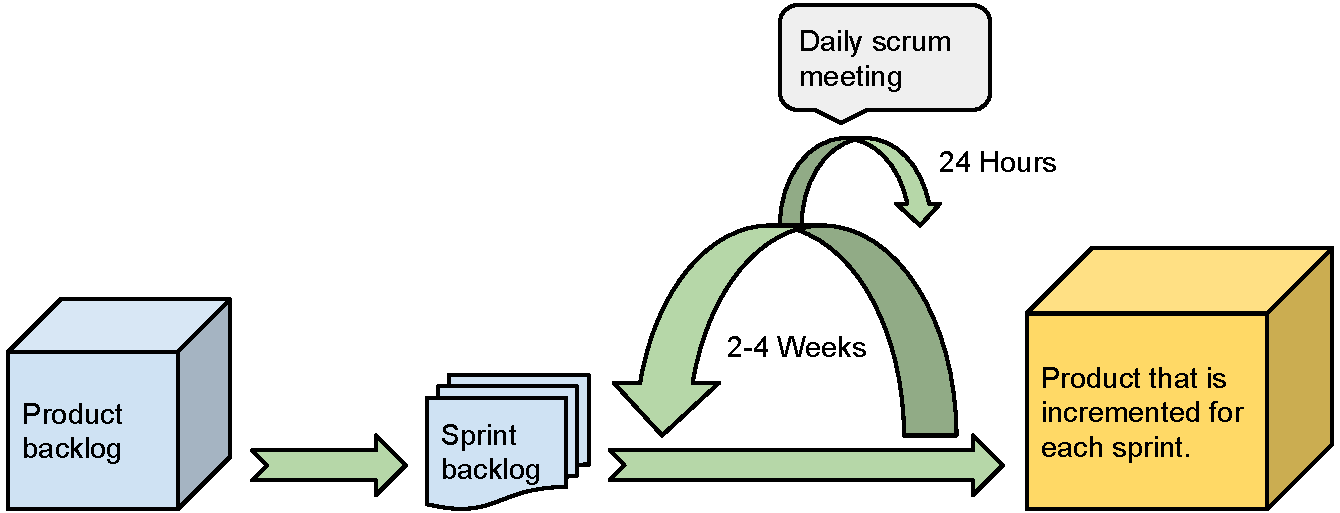
\includegraphics[scale=0.5]{../Figures/Scrum-workflow.pdf}
\end{center}
\caption{Scrum workflow}
\label{figure:scrum-workflow}
\end{figure}

%-----------------------------------
%	SUBSECTION 3
%-----------------------------------
\subsection{Conclusion}
\label{subsec:devprocess}

After discussing about possible alternatives, we decided to use Scrum based on the following considerations:

\begin{enumerate}
\item we didn't have a formal set of requirements from the beginning and we expected their nature to be volatile,
that is, subject to change throughout the duration of the project.

\item at the beginning of the project, our knowledge of both the problem and the technologies involved was
limited thus it would have been very risky to make decisions we wouldn't be able to adjust later.

\item given the size of the project and of our group, we wanted a development process with a small overhead.
Waterfall is notoriously not a process with a small overhead.

\item we had previous working experiences with Scrum, whereas our experience with Waterfall was only theoretical.

\item the customer suggested us to use an agile method.

\end{enumerate}

All in all, Scrum seemed to fit very well the nature of this project.
We thought that iterating the same activities over and over would have led to a natural improvement of our process and left a lot of possibilities to adjust the requirements and thus the design accordingly.
However, we made the following adjustment to the process in order to adapt it to our specific case:

\textbf{Daily scrum}\newline
We performed daily scrum on days we planned to work together: Mondays and Wednesdays.
Because everyone in the group had to attend courses, or to deliver assignments, or a job, or all these things, we couldn't work every day on the project. 
Since there was nothing to report, we didn't see the need for a daily scrum meeting.

\textbf{Sprint review meetings}\newline
Usually this meeting is held at the end of a sprint. 
In our case however, because our last meeting each week was on Wednesdays but we often worked on the project later during the rest of the week, we decided to combine the sprint review meeting with the sprint planning meeting (on Mondays every two weeks).


\section{Existing Solutions}
\label{section:existing-solutions}

This section describes existing solutions which have helped us get a better overview of technologies
and design patterns used to solve this kind of problem. 
What we present in this section are the ones we found most relevant and inspiring for our work.

%-----------------------------------
%	SUBSECTION 1
%-----------------------------------
\subsection{HealthVault}
%http://msdn.microsoft.com/en-us/healthvault/jj128027

HealthVault\cite{HealthVault} is Microsoft's online platform to collect, store and monitor personal health information. 
One of its most interesting features is interoperability with third-party solutions which are,
in HealthVault terminology and in this subsection hereafter, referred to as \textit{Apps}.

Examples of Apps include:
\begin{itemize}
\item smartphone and desktop applications
\item devices like step counters, blood glucose meters, weighting scales\ldots
\item third-party health services like Withings, \ldots
\end{itemize}

At the moment of writing, HealthVault supports more than 300 applications and 80 devices (in the U.S.).
Apps are used to populate a user's health record by collecting health measurements and parameters and, in turn,
make use of such information to provide services.
In order to connect to HealthVault, third-party applications need to be authorized by the user upon first use. 
Authorization can be restricted to a specific set of data: e.g. an App may be authorized to access weight and
glucose records but not allergies and pregnancies.

Thanks to a well documented XML-over-HTTP API and several software development kits (SDK)
for major mobile platforms and languages, it is easy for third-party developers to implement
interoperability with HealthVault in their application.

The API defines a set of data called \textit{things}.
Basically, a \textit{thing} represents a measurement of some health parameter e.g. heart rate, weight.
\textit{Things} are represented using XML, see an example below (a weight \textit{thing}).

\begin{lstlisting}[language=XML]
<weight>
  <value>
    <kg>60</kg>
    <display units="kg">132</display>
  </value>
  <when>
    <date>
      <y>1990</y>
      <m>1</m>
      <d>1</d>
    </date>
    <time>
      <h>1</h>
      <m>0</m>
      <s>0</s>
    </time>
  </when>
</weight>
\end{lstlisting}

Additionally, HealthVault supports exporting of data in industry-standard formats and storage of medical
imaging formats such as \textit{DICOM} and provides a degree of availability and redundancy.
Figure \ref{figure:hv-page} shows Ola Nordmann HealthVault's web page.

\begin{figure}[h]
\begin{center}
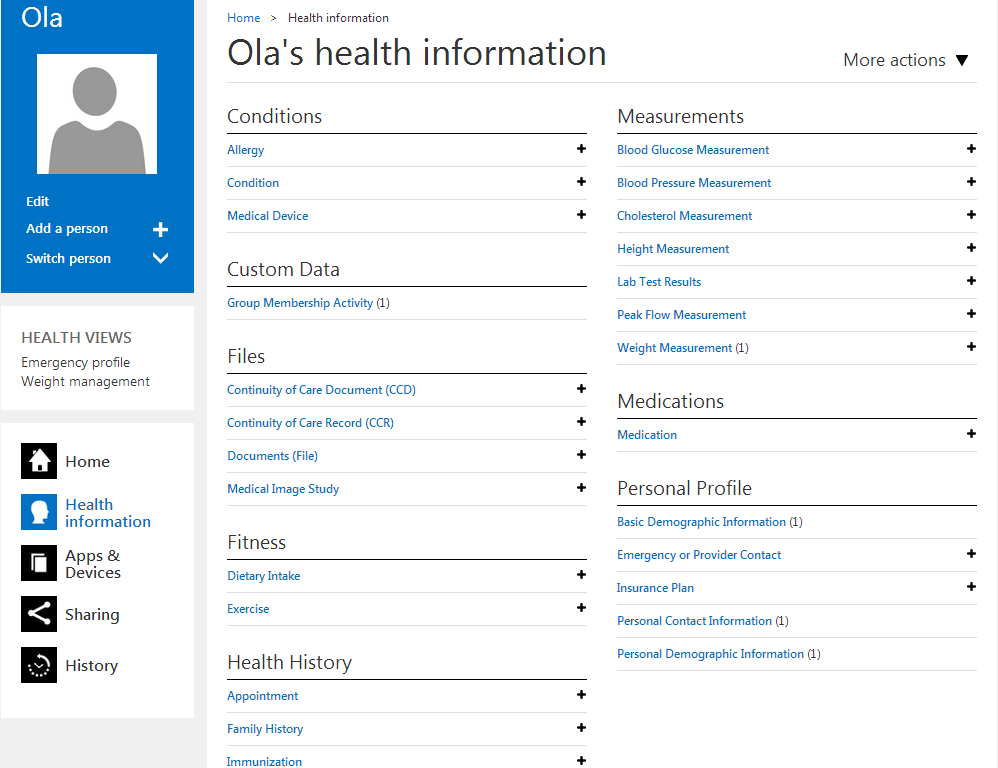
\includegraphics[scale=0.50]{../Figures/hv-page.png}
\end{center}
\caption{HealthVault web interface}
\label{figure:hv-page}
\end{figure}

%maybe we cant use this picture. it's good tho...
\iffalse
\begin{figure}[h]
\begin{center}
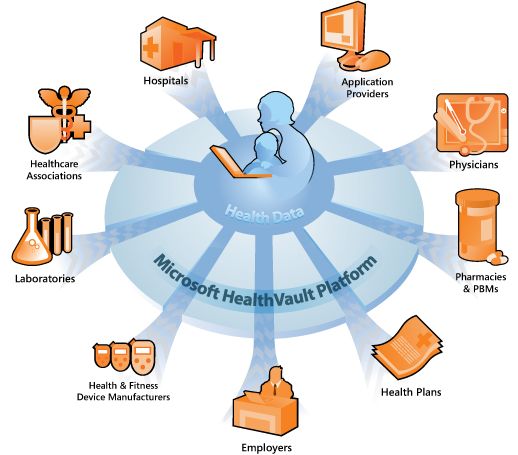
\includegraphics[scale=0.6]{../Figures/hv-cloud.png}
\end{center}
\caption{HealthVault apps}
\label{figure:hv-apps}
\end{figure}
\fi

%An HealthVault account can be linked to multiple individuals.

%-----------------------------------
%	SUBSECTION 2
%-----------------------------------
\subsection{human/api}
\label{section:humanapi}

The human/api is a RESTful web API for health data developed by human/api Inc.
Its aim is to offer a single access point to people's health information in order to facilitate developing
health applications. For this purpose, human/api collects people's health parameters (blood pressure, weight\ldots)
from a variety of third-party services (e.g. Withings) and devices (e.g. sensors) and normalizes it.
The data is then made available through a clean and well documented web API.
This has the benefit of providing a single service for application developers to authenticate against in order
to obtain users' health information, without having to integrate with multiple services individually.
Additionally, all data is represented using standardized models and format (JSON) of which we present an
example below. \cite{HumanAPI}

\begin{lstlisting}[language=JSON]
{
  "id": "string",
  "userId": "string",
  "time": "date",
  "value": {
    "diastolic": "int",
    "systolic": "int",
    "unit": "string"
  },
  "heartRate": "int"
}
\end{lstlisting}

%-----------------------------------
%	SUBSECTION 3
%-----------------------------------



%-----------------------------------
% SUBSECTION 4
%-----------------------------------
\subsection{Open eHealth Foundation}

The goal of Open eHealth Foundation is to create and share open source software components for the healthcare ICT industry.
One of their products is an integration platform called Open eHealth Integration Platform (IPF).
It is based on Apache Camel and has support for connecting systems in the eHealth domain. \cite{OpenEHealthFoundation}


%-----------------------------------
%	SUBSECTION 5
%-----------------------------------
\subsection{Conclusion}

The solutions presented in this subsection were of great influence in our work.
\verb|human/api| influenced our data models and representation as well as being a good example of how to implement security.
HealthVault, together with its SDKs proved to be a valuable example of a modern health integration platform.
We made use of HealthVault SDK to interact with the Microsoft's platform and were able to re-use a large portion of the code shipped as example.

%The android-heart-rate-monitor application was used to provide functionality that would have
%taken some effort to implement from scratch.


\section{Security concerns}

This section describes our studies about security.

\subsection{HIPAA - Health Insurance Portability and Accountability Act}

\begin{figure}[h]
\centering
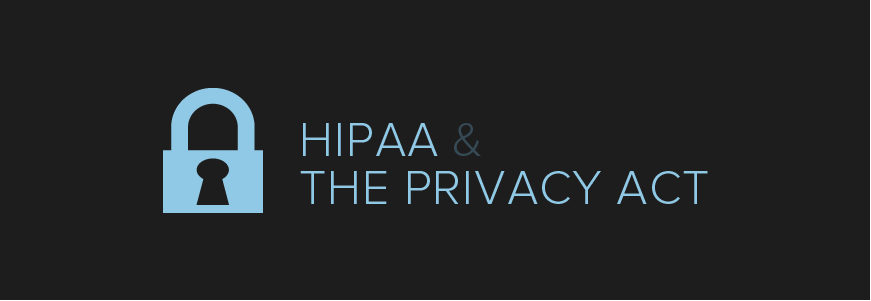
\includegraphics[scale=0.50]{../Figures/hipaa2.png}
\caption{HIPAA logo}
\label{figure:HIPAA}
\end{figure}

HIPAA\cite{HIPAA} is an American act which, among other things, establishes some standards
for electronic health care. The \textit{privacy regulations} in HIPAA require
that a set of practices and precautions is put in place when transferring, sharing
and handling health information electronically.
After discussing security with the customer we brought up the topic of HIPAA.
Even though there is no similar act in Norway, the customer believed that it could have been
valuable to discuss it and take it as starting point for our considerations about security. 

\textbf{Storage of data}\newline
HIPAA specifies that the hard drives used to store data must be encrypted and
kept safe from unauthorized physical access. HIPAA does not specify what type
of encryption should be used.

\textbf{Transfer of data}\newline
Data transfer should be carried out using a Secure Socket Layer\cite{SSL}
to prevent access by unauthorized people by means of encryption.

\textbf{Backup of data}\newline
Data should be backed-up in a exact and retrievable copies.
The frequency of backups should be appropriate for the data itself
taking into consideration how often is said data being updated and how it is being
used.

\textbf{Logging}\newline
Data access has to be logged in order to be able to monitor who
has accessed what and when.

\textbf{Security breaches}\newline
If a security breach happens, people whose data could have been compromised
should be notified. Depending on the severity of the breach, which could be
based on the amount of information disclosed or their sensibility,
a public announcement must be made.

\textbf{Authorization}\newline
HIPAA specifies that the user must be able to authorize access to his data,
which must be requested specifying not only the data itself, but also
an expiration for the requested authorization, its purpose and all parties
which request such authorization.

\subsection{Authentication}

There are multiple systems already in use in Norway for authenticating users. 
Some of the biggest systems are MinId, BankID, Buypass and Commfides.
The most widespread is BankID, with almost 3 million users at the moment
writing\footnote{See https://www.bankid.no}.
It would be worth considering to use BankID to authenticate citizens because
it is already adopted by most of them.


\subsection{OAuth 2.0}

OAuth 2.0\cite{OAuth} is a standard for authorization. %third-party applications to access data on a system.
%securing that could potentially be used for our integration platform.
%OAuth 1.0 is outdated, and hence we will mainly focus on OAuth 2.0 in this section.
%OAuth is used to authorize third party applications access to a system.
%In our case this could for example be only access to the API concerning heart rates or weights in NIPEN.

%\subsection{What is OAuth?}

The scenario where an application wants to interact with an API provider to obtain information
about a user is becoming more and more common: think of Facebook and all the applications that use data
which Facebook provides. It would certainly be a bad idea for a user to share his account credentials
with many third-party applications because doing so would enable them to do what they want with it.

\iffalse
% the user doesn't always want to give his/hers credentials to these applications.
Lets say that a user wants user an application that is able to upload images to his/hers
Facebook account but doesn't feel confident about giving the applications his Facebook credentials.
%The user doesn't want to give the application the credentials for facebook.
This would be highly insecure, since once the application has the authentication information
of a user it is able to do whatever it wants with the account.
\fi

OAuth tries to solve this kind of problem authorizing third-party applications to access
user's information, or part of it, on a server without providing any account credentials.

For this purpose third-party application developers need to register their application
with the API provider. This might include name of the application, a description, logo\ldots
This is to allow applications to be authenticated and controlled by the API provider itself.
Upon registration, a client-ID to be used for authentication is assigned to the application.

Then, in order to be authorized to access some user's data, the application redirects the
user to the API provider's page where he can authenticate himself without actually providing
any credentials to the application. Then he proceeds to authorize the application to access (or not)
a specific set of data. The application is finally returned a token representing the level
of authorization granted. Authorization can be revoked by the user at any time.


%For this purpose it makes use of a token based system, where the application receives a token specifying
%the authorization level granted to it by the user.

%A redirect URI also needs to be registered.
%This URI needs to use TLS, i.e. must begin with \textit{https}.
%This address is used to send an authentication token from the system to the application.
%After the registration, the application should receive a client ID which is used to identify the application at the system.
\iffalse
Now users should be able to connect the application with theirs account on the system.
The way it works is that through the application they will be sent to a website of the system the application wants to connect with.
There the user will be asked if he/she wants to grant permissions to the application.
If the user agrees, then he/she will be redirected to the applications specified redirect URI with an access token as a parameter.
The application will now use this token to access the system.
When the user doesn't want the application to have access to the system any more, he/she can simply disallow the applications access through the systems website.
\fi

An example of how OAuth works is given in figure \ref{figure:oauth-in-a-nutshell}.
In this example we see a website that wants to send images to a user's Facebook account.
If the user authorizes the application through Facebook, then Facebook will send an access
token to the website. Then \textit{www.ImageToFacebook.com} will be able to send images to the
users account, providing their access token for authorization.
%The user should be able to disallow the website access at any time on Facebooks website. 

\begin{figure}[h]
\centering
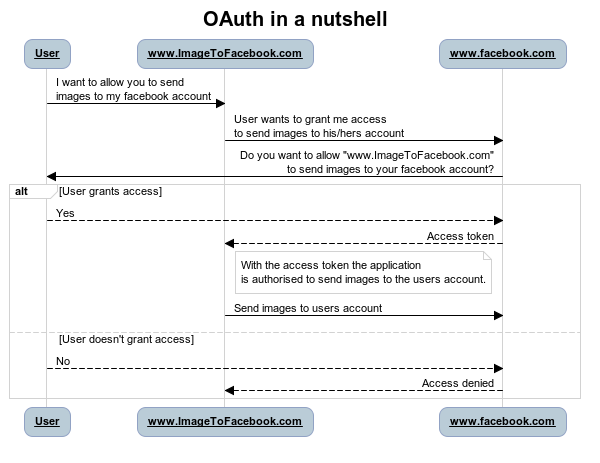
\includegraphics[scale=1.0]{../Figures/oauth-in-a-nutshell.png}
\caption{OAuth in a nutshell}
\label{figure:oauth-in-a-nutshell}
\end{figure}


\clearpage
%----------------------------------------------------------------------------------------
%	SECTION 4
%----------------------------------------------------------------------------------------
\section{Involved technologies}
\label{section:used-technologies}

In this section we present some relevant technologies we took into consideration for our product.

%-----------------------------------
%	SUBSECTION 1
%-----------------------------------
\subsection{Programming languages}

\textbf{Java}\cite{Java}\newline
Java is a general-purpose programming language that it can be used in a wide variety of application domains.
It is platform independent, and thus makes it easy to develop software once and deploy it on different operative systems.
Web programming is one of the domains that Java is used in, making it possible to write a service
that runs in the back-end of a website (using JSP).
%The web services created with Java allows creating a bridge between the database and the front-end. 
%This makes it possible to create a communication between the user and the database at the server.


%-----------------------------------
%	SUBSECTION 2
%-----------------------------------
\subsection{Database}
In this section we present those technologies related to database development.

\textbf{MySQL}\cite{MySQL}\newline
MySQL is one of the most widely used relational database management system.
The Community Edition of MySQL is open source and freely available.
It is developed to handle large databases and support many users at the same time.%. and it is also scalable.
It makes it possible to store and retrieve data in an efficient and structured manner. 

\textbf{Microsoft SQL server}\newline
Microsoft proprietary SQL server implementation. Needless to say, it only runs of Microsoft
Windows. A freeware \textit{Express} version is available.

\textbf{Apache Derby}\newline
Apache Derby is a relational database management system developed by the Apache foundation
and released under the Apache License 2.0.

\textbf{MySQL Workbench}\newline
MySQL Workbench is a free-to-use tool which allows to easily manage MySQL databases.
We used MySQL Workbench for database design and deployment both locally (for testing) and remotely (production).


%-----------------------------------
%	SUBSECTION 3
%-----------------------------------
\subsection{Web development}
In this section we present those technologies related to web development.

\textbf{Spring Framework}\cite{SpringFramework1}\cite{SpringFramework2}\newline
The Spring Framework is an a Java-based application framework and inversion of control container.
Spring is widely used and freely available under Apache License 2.0\footnote{See http://www.apache.org/licenses/LICENSE-2.0}.
%We use the Spring framework to set up a RESTful service and to handle the data access from the database. 

\textbf{Apache Tomcat}\cite{ApacheTomcat}\newline
Apache Tomcat is a mature, reliable and freely avaialable HTTP web server implementation licensed
under the Apache License 2.0. Additionally, Apache Tomcat runs on a variety of different platforms.
Numerous companies and organizations use Apache Tomcat for large-scale and mission-critical web applications.

\textbf{Microsoft IIS}\cite{}\newline
Microsoft Internet Information Services (IIS) is Microsoft's proprietary web server solution.
It is stable, mature and well documented. It is shipped as an integral part of Windows operative system (sharing thus
its same license), although a freeware, stand-alone version is also available. Needless to say, Microsoft IIS only
runs on Windows.

\textbf{Microsoft WCF}\cite{}\newline
Microsoft's WCF is Microsoft's framework for developing applications that communicate over a network.
WFC uses Microsoft's proprietary .NET framework to develop web applications.

\textbf{HTML5}\cite{HTML5}\newline
HTML is the standard World Wide Web's markup language, HTML5 being the latest HTML version at the moment of writing.
It is used to structure and visualize web pages on the internet. By writing a document with HTML a
web browser is later on able to interpret the document and visualize it in a structured manner. 

\textbf{CSS3}\cite{CSS3}\newline
CSS describes the look and format of a document written in HTML.
It allows one to use different fonts, colors and adjust the layout of a web page.
By using CSS and separating it from the HTML, it is possible to allow multiple pages share the same style
making them easier to maintain and adapt to different environments. 

\textbf{Bootstrap}\cite{Bootstrap}\newline
Bootstrap contains HTML and CSS templates for web designers.
This makes it easier to make a good looking web page without putting too much effort into the design.

\textbf{JavaScript}\cite{JavaScript}\newline
JavaScript is an interpreted computer programming language that runs in the browser of the user.
It is allowed to make changes in the HTML DOM, interact with the user, control the browser and communicate asynchronously.
Since it can communicate with the server asynchronously, it makes the web page more dynamic.
What this means is that a web page can acquire new information and change the site without reloading.

\textbf{jQuery}\cite{jQuery}\newline
jQuery is a JavaScript library for manipulating and traversing the HTML DOM.
All the features available in jQuery are achieved using pure JavaScript, but jQuery helps
the developer to implement the different features in an easier way:
e.g. it contains predefined methods for event handling and animation.
It also makes it easier to communicate with the server through AJAX. 

\textbf{Chart.js}\cite{Chartjs}\newline
Chart.js is a JavaScript library for creating graphs and charts.
It helps the developer to easily visualize data through different types of graphs.
The library has support for different types of two dimensional data, e.g. value per time.
It also has the ability to display multiple graphs in the same chart. 


\subsection{Mobile Technologies}
In this section we present those technologies related to mobile development.

\textbf{Android SDK}\cite{AndroidSDK}\newline
The Android SDK contains the tools necessary for developing, debugging and testing a Android applications.
%With the SDK it is possible to write and modify applications for an Android phone.

\textbf{android-heart-rate-monitor}\cite{AndroidHeartRateMonitor}\newline
\label{subsec:hr}
android-heart-rate-monitor is an open source (Apache 2.0 license) Android application that can be used to measure
the user heart rate. The application uses the phone's camera and flash to compute 'redness' levels on user's fingertips. 
These are supposed to increase in correspondence with heartbeats. The application computes an average 'redness' value
and uses that to detected heartbeats and calculate a beats per minute (BPM) measurement.


%% redudant with tools section. they are tools not really 'technologies'

\iffalse
\subsection{Other Technologies}

\textbf{Maven}

Maven is a software tool for managing a programming project.
It has the ability to build and compile programming code based on the content of a POM (Project Object Model) file.
It keeps track of all the frameworks used, and is able to download them before building the project. \cite{Maven}

\textbf{Git}

Git is a version control system that is free and open source.
This is an important tool to keep track of all the changes made to the source code, it also makes it easier for multiple developers to work on the same source.
Git makes it easy to roll back changes made to the code, in case something was wrongly implemented.
It also has the possibility to divide the project into different branches.
Which means that the code can be copied into multiple different places, and developed separately in cases where trying out different solutions is necessary.
If a good solution is made, the branch can later on be merged together with the main branch.
It is also possible to have a branch for release versions and a development branch. \cite{Git}
\fi

\subsection{Conclusion}

There were, of course, a number of alternatives to most of these technologies and the whole
report wouldn't be enough to describe them all. The reasons behind our choices have been very practical.
We didn't want, if possible, to limit our product to one single platform so we chose to avoid Microsoft's solutions.
Additionally, we were limited to those solutions which were freely available to us.
We tried, when possible, to opt for technologies which were well documented and that we were not
totally unfamiliar with in order minimize the time we would spend to figure out how to make them work.
We don't claim that our choices of employed technologies are the 'best' choices possible,
but we found them appropriate for our case.

\iffalse
We chose the technologies specified above based on our earlier experience and what we found most appropriate for our solution.
Before we started this project we discussed our competencies.
This was of great help in choosing the right technologies that were going to be used.
Most of us already had some different degree of experience in most of the technologies mentioned above.
This made it much easier for us to chose the right set of frameworks and languages to work with.
\fi

%----------------------------------------------------------------------------------------
%	SECTION 5
%----------------------------------------------------------------------------------------
\section{Service oriented architectures}

The architecture of the service itself will play an important factor in its scalability and complexity.
In this section we will cover some methods that can be used for interaction between clients and servers. 

\subsection{REST}
\label{subsec:rest}

\cite{REST} REST, is an acronym from Representational State Transfer and is basically an architectural style where clients
(user agents) make requests of services (endpoints) to servers.

REST is based on a set of principles:
\begin{itemize}
\item Clients interact with resources. The term 'resource' refers to anything that can have a name and a representation.
      A resource is addressed via a unique Uniform Resource Identifier (URI).
\item All informations regarding a resource are contained in the resource itself: resources are self-descriptive.
      Because all information needed to process a request on any resource is contained in the resource itself,
      the services can be stateless.
\item Resources can be accessed by client using HTTP methods such as \verb|GET|, \verb|POST|, \verb|PUT| and \verb|DELETE|.
      Each of these methods corresponds to an operation:
			\begin{itemize}
				\item \verb|GET|: returns all the elements of a collection, or a specific element if its ID is specified.
				\item \verb|POST|: creates a new entry in a collection or a new element.
				\item \verb|PUT|: is to replace a collection or a particular element in it.
				\item \verb|DELETE|: deletes an entire collection or a particular element in it.
			\end{itemize}
\item Resources can contain link to other resources.
\end{itemize}

This type of service does not have any specific requirements on how the data should be formatted or what it should look like.
What described, results in a number of advantages.

\textbf{Scalability}\newline
Because RESTful services are stateless, they are generally lightweight in resources and easy to scale up.

\textbf{Caching}\newline
Requests sent to RESTful services are made using HTTP methods and HTTP \verb|GET| results are cached, this can
lead to further scalability capabilities and speed.

\textbf{Interoperability}\newline
REST only requires an HTTP connection.

\textbf{Idempotency and nilpotency}\newline
%\verb|PUT| and \verb|DELETE| methods are idempotent. This means that one nullifies the effects of the other.
\verb|PUT| and \verb|DELETE| methods are idempotent. 
This means that after executing these methods once, later execution of this methods will have no effect.
Because an element can only be replaced or deleted once.
\verb|GET| is nilpotent, meaning that it has no side effects. These are desirable features considering
that over a network information is likely to get lost or sent multiple times and it would not unlikely for an operation
to be executed twice. %Having the possibility to revert changes made to the data could be valuable,
%as well as having a nilpotent operator that has no effect on data itself.

\textbf{Simplicity}\newline
REST is simple and that is one big advantage.

\subsection{SOAP}\cite{SOAP}
\label{subsec:soap}
SOAP (Simple Object Access Protocol) is a protocol for exchanging information between web services in a network.
SOAP makes heavy use of XML for communication. There are strict rules on how the XML data should be formatted.
A SOAP message consists of different parts: a header, a body, a fault and an envelope. Some of these
are mandatory while some are optional. Table \ref{table:soap-message} shows an overview of these parts.

\begin{table}[h]
\begin{center}
\begin{tabular}{ | l | l | c | }
  \hline
  Part  & Description & Required \\
  \hline\noalign{\smallskip}\hline
  Header & Contains header informations & No \\
  Body   & Represents the body of the message   & Yes \\
  Fault  & Describes eventual errors occurred during processing  & No \\
  Envelope & Wraps the whole message & Yes \\
  \hline
\end{tabular}
\end{center}
\caption{SOAP message parts}
\label{table:soap-message}
\end{table}

The structure of a SOAP message is illustrated in figure \ref{figure:soap-message}.

\begin{figure}[h]
\begin{center}
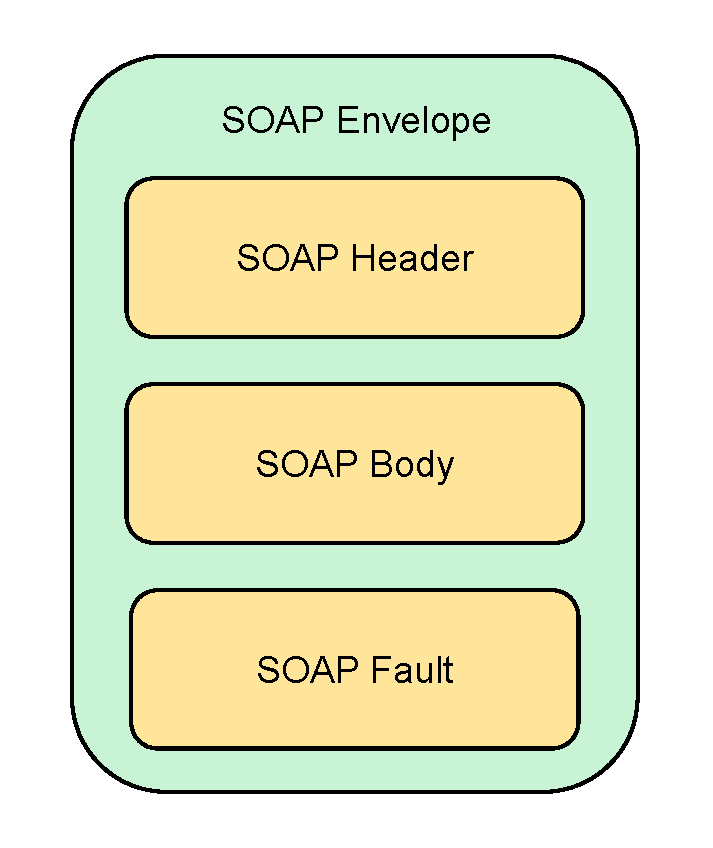
\includegraphics[scale=0.50]{../Figures/SOAP.pdf}
\end{center}
\caption{SOAP message structre}
\label{figure:soap-message}
\end{figure}


%It needs to contain an envelope and a body, in addition it can also contain a header and a fault.
%The envelope tells that the message that is being sent is a SOAP message, and the body contains the main information
%that is being sent. A header can contain header information, and fault tells if there were some errors during the
%processing of the message. Figure \ref{} shows a SOAP message.

SOAP has three major characteristics:
\begin{enumerate}[1.]
\item it is neutral, in the sense that it doesn't specify a mean to transport data
\item it is independent, meaning that it allows for any programming model
\item it is extensible
\end{enumerate}

Furthermore, it has a number of advantages over over other formats like pure XML and JSON:
\begin{itemize}
\item SOAP messages can have multiple recipients
\item parts of a SOAP message can be encrypted to be readable by certain recipients only
\item SOAP allows to represent more generic data structures
\item SOAP messages are guaranteed to be delivered
\end{itemize}

\subsection{Conclusion}
\label{subsec:soa-conclusion}
All in all, we found REST more suitable for our product for a number of reasons.
In the first place, REST is simpler than SOAP and we didn't need all the complexity introduced by the latter.
Additionally, REST is generally considered more lightweight due to its use of a less verbose data
represention (JSON vs XML). Both these factors contribute to a better scalability.
We were sure that REST would be available on any platform since what is needed
is really only an HTTP library. Furthermore, we all had some kind of experience with
REST APIs but none of us never had any experience with SOAP.

%Since SOAP uses XML and has strict rules for how the data format should be, we find a
%RESTful service more appealing for our solution.
%With rest it is possible to send raw JSON strings with a custom defined format.
%JSON strings are much easier to handle and manipulate on a web based front-page, by using JavaScript.

%----------------------------------------------------------------------------------------
%	SECTION 6
%----------------------------------------------------------------------------------------
\section{Testing}
\label{section:testing}

%In this section we are going to go through some of the testing frameworks used in our project.
In this section we are going to go through some of the testing frameworks explored during our preliminary study.

\subsection{JUnit}

JUnit is a Java framework for writing tests. It is also a good tool when using test driven development.
With help of this framework it is possible to write tests for different parts of the code, then check if it runs as it should.
It is also possible to use JUnit with Maven.
When doing so it will first run all the tests, and if the tests are successful the application will be executed. \cite{JUnit}

\subsection{Jasmine}

Jasmine is a framework for testing JavaScript code.	
It doesn't require a DOM and is also not dependent on any other frameworks. \cite{Jasmine}

\subsection{Conclusion}

When using test driven development it is important to have some frameworks for testing the code.
New bugs are often introduced to applications when extending it with new functions and features.
With help of the technologies mentioned above it is much easier to find the new bugs, and hence fix them quicker.